\section{Case Study}
\label{sec:case_study}

This section presents a case study comparing three methods to determine the harmonic hosting capacity of a phase-balanced three-phase power system, using the IEEE 30 bus test system~\cite{shahidehpour_appendix_2003}. First, the necessary technical assumptions for the methods are enumerated. Second, the harmonic hosting capacity is determined for a network with overhead lines based on the three methods. Lastly, the impact of underground cable connections on the harmonic hosting capacity is investigated. Due to space limitations, it is impossible to show all resulting individual harmonic unit currents and bus voltages for all three methods, consequently, specific results are selected to support the conclusions. However, the case study has been made available in \textsc{HarmonicPowerModels.jl}
% as a \textsc{Pluto}-script in the example folder of .

\subsection{Technical Assumptions}
\label{sec:technical_assumptions}

For consistency the individual harmonic voltage limits~$\VoltageParameter^{\text{ihd}}_{\Harmonic}$ denoted in IEEE519:2022 are used for all three methods. 
%Table~1
\subsubsection{Look-Up Method Following Std. IEEE519-2022}
To look-up the relative individual harmonic current limits~$\CurrentParameter^{\text{ihd}}_{\Unit,\Harmonic}$, the nodal three-phase short-circuit current is required. They are calculated under following assumptions:
\begin{enumerate*}
    \item [a)] no short-circuit contribution of the load units, and
    \item [b)] generator short circuit power is chosen to be 2.1GVA for all generators, with a XR-ratio of 20.
\end{enumerate*}

\subsubsection{Analytical Method Following Std. IEC61000-3-6:2008}

To most-clearly illustrate the difference between a nodal and a full network approach to determine the harmonic hosting capacity, all harmonic influence factors~$K_{ij,h}$ are set to one. Furthermore, the reader is reminded that no harmonic recombination is assumed, consequently, all parameters~$\alpha$ related to the general summation law are set to one.

\subsubsection{Novel Optimization Method}
To be consistent with all other methods, root-mean-square or total harmonic distortion limits are not enforced. Furthermore, the absolute equality is enforced between all units, consequently, all individual harmonic current injection for all units will be equal.

\subsection{Case A: Overhead Line Network}

This section presents the results for a network with overhead line connections comparing the three methods in terms of individual harmonic current injection~$\Current^{\text{ihd}}_{\Unit,\Harmonic}$ by the units and the resulting individual harmonic bus voltage~$\Voltage^{\text{ihd}}_{\Node,\Harmonic}$. All shunt susceptances of the branches in the test case are set to zero to obtain a network impedance exhibiting no resonances and increasing monotonically for the considered frequency range. The nodal harmonic impedance of high-voltage bus~4 and medium-voltage bus~17 are illustrated in Fig.~\ref{fig:nodal_impedance}.

Fig.~\ref{fig:i_ihd_ind} shows the individual harmonic current injection~$\Current^{\text{ihd}}_{\Unit,\Harmonic}$ by the units for all three methods and Fig.~\ref{fig:u_ihd_ind} shows that the presented optimization approach best utilizes the prescribed individual harmonic voltage limits. The IEEE519-2022 method results in harmonic voltages exceeding the prescribed limits at certain harmonics for the medium-voltage bus~17 wheras, the IEC61000-3-6:2008 method results in harmonic bus voltages significantly lower than the prescribed limits. Consequently, in cases with no resonances, the presented optimization method best utilizes the harmonic hosting capacity of the network without violating any individual harmonic voltage limit.

\begin{figure}[b!]
\centering
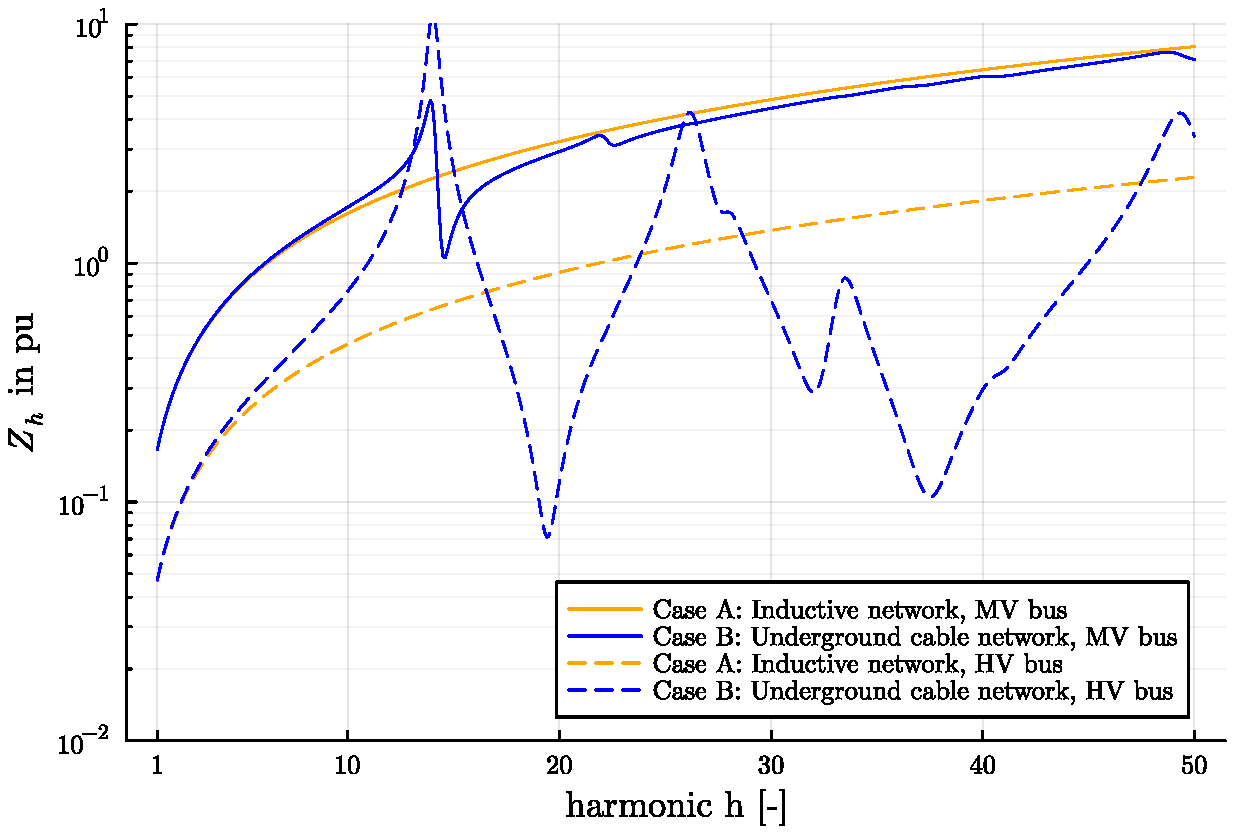
\includegraphics[width = 0.9\columnwidth]{figures/zh.pdf}
\caption{Nodal impedance of medium-voltage bus~17 (solid lines) and high-voltage bus~4 (dashed lines), considering a) a network with overhead line (blue line), and b) a network with underground cable connections (orange line).}
\label{fig:nodal_impedance}
\end{figure}

\subsection{Case B: Underground Cable Network}

This section presents the results for a network with underground cable connections for all three methods, in terms of individual harmonic current injection~$\Current^{\text{ihd}}_{\Unit,\Harmonic}$ by the units and the resulting individual harmonic bus voltage~$\Voltage^{\text{ihd}}_{\Node,\Harmonic}$. All shunt susceptances of the edges are restored to the original data in the IEEE 30 bus system. This adds a number of resonances to the nodal harmonic impedance, as shown in Fig.~\ref{fig:nodal_impedance}. Given that all underground cable connections are at the high-voltage level, these resonances are significantly more pronounced for the high-voltage bus~4 compared to the medium-voltage bus~17. 

Fig.~\ref{fig:i_ihd_cap} shows the individual harmonic current injection~$\Current^{\text{ihd}}_{\Unit,\Harmonic}$ by the units for all three methods. It can be seen that all methods except for the IEEE519-2022 accounts for the harmonic impedance resonances in the system. Similar as in the previous case, Fig.~\ref{fig:u_ihd_cap} shows that the presented optimization approach best utilizes the prescribed individual harmonic voltage limits. The IEEE519-2022 method results in harmonic voltages exceeding the prescribed limits at certain harmonics for both the medium-voltage bus~17 and high-voltage. Around the resonance frequency, the IEC61000-3-6:2008 method also results in harmonic voltages exceeding the prescribed limits whereas elsewhere the harmonic bus voltages remain significantly lower than the prescribed limits. Consequently, in the context of a network exhibiting resonances, the presented optimization method again best utilizes the harmonic hosting capacity of the network without violating any individual harmonic voltage limit.

\begin{figure*}
\centering
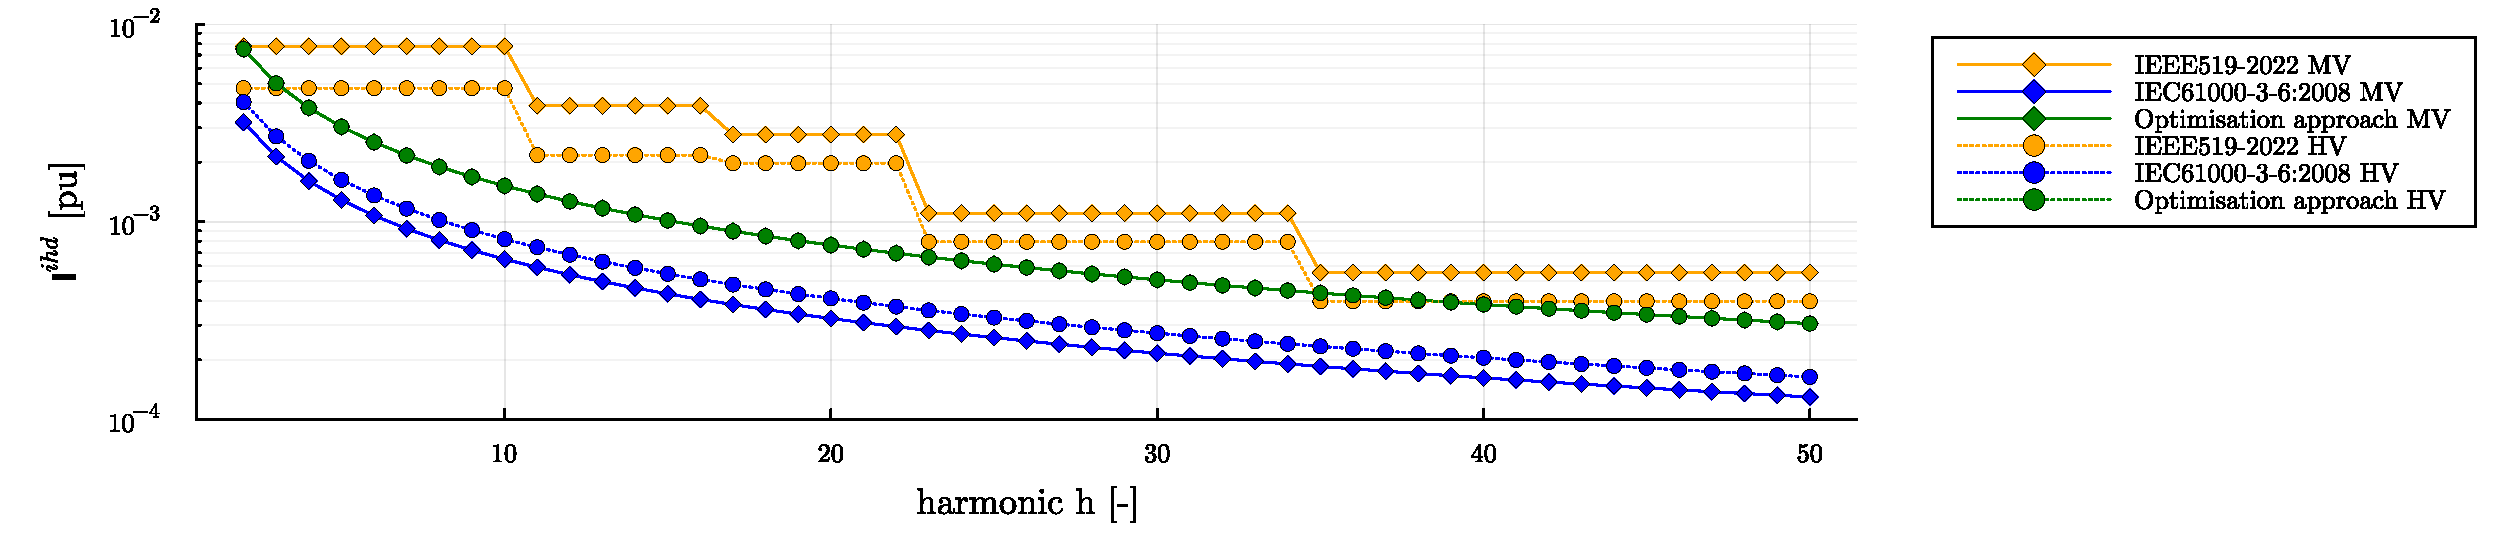
\includegraphics[height=3.5cm]{figures/ihd_ind.pdf}
\caption{Case A: overhead line network -- individual harmonic current~$\Current^{\text{ihd}}_{12,\Harmonic}$ of unit~12 at medium-voltage bus~17 (solid lines w. diamond marker) and~$\Current^{\text{ihd}}_{3,\Harmonic}$ unit~3 at high-voltage bus~4 (dotted lines w. circle marker), using one of three methods: a) IEEE519-2022 (orange), b) IEC61000-3-6:2008 (blue), and c) novel optimization method (green). Note that the curves for the optimization method (green) overlap due to the chosen absolute equality fairness principle.}
\label{fig:i_ihd_ind}
\end{figure*}

\begin{figure*}
\centering
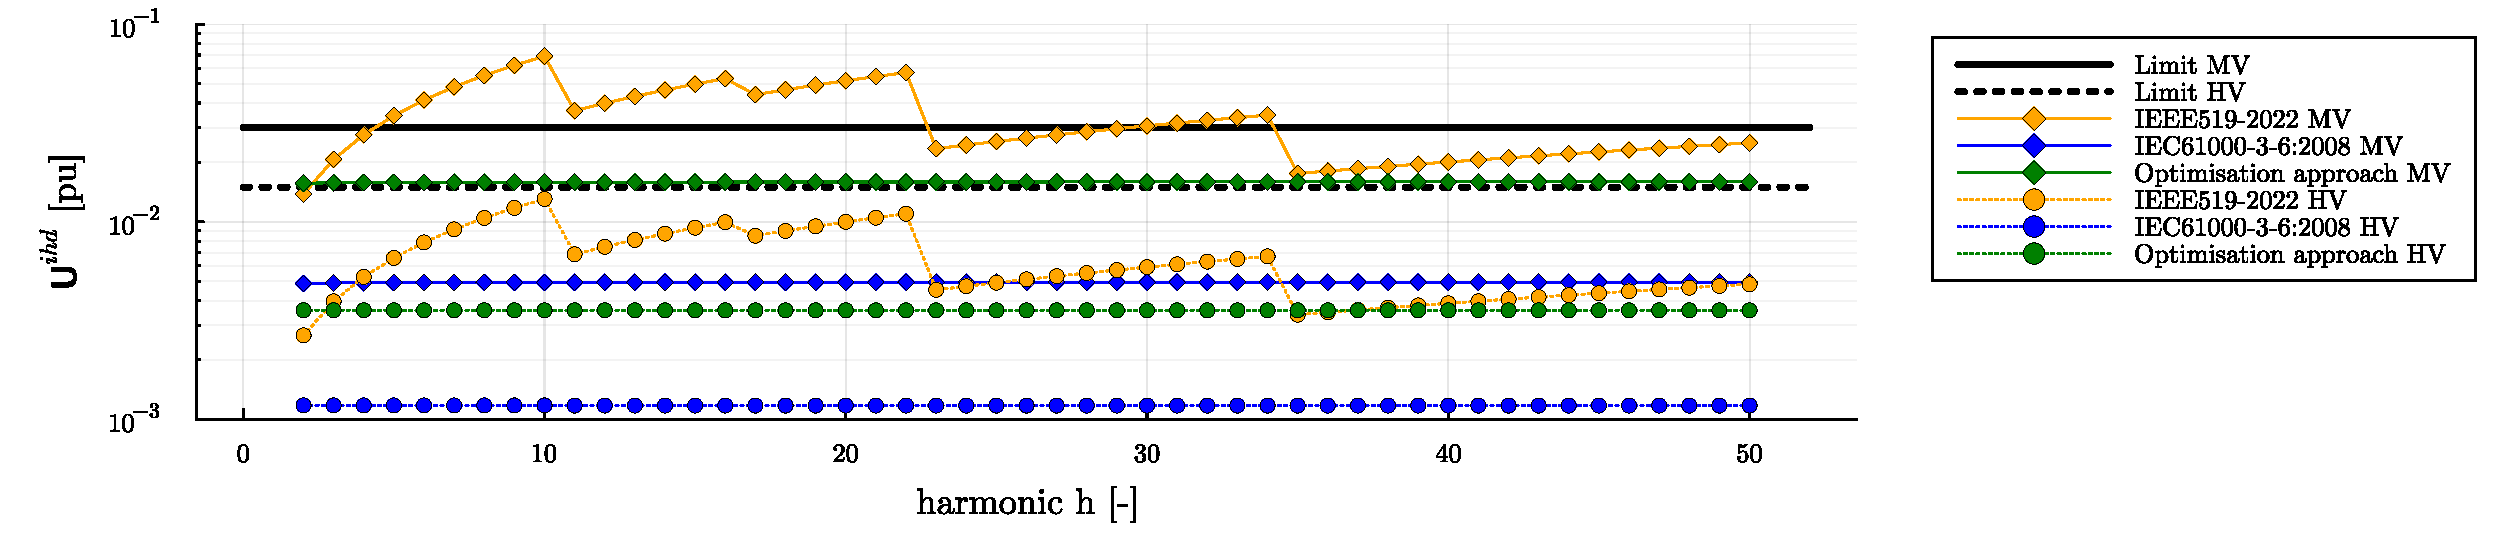
\includegraphics[height=3.5cm]{figures/uhd_ind.pdf}
\caption{Case A: overhead line network -- resulting individual harmonic voltage~$\Voltage^{\text{ihd}}_{17,\Harmonic}$ at medium-voltage bus~17 (solid lines w. diamond marker) and~$\Voltage^{\text{ihd}}_{4,\Harmonic}$ at high-voltage bus~4 (dashed lines w. circle marker), following a harmonic power flow based on the injected harmonic unit current determined using one of three methods: a) IEC61000-3-6:2008 (blue), b) IEEE519-2022 (orange), and c) novel optimization method (green).}
\label{fig:u_ihd_ind}
\end{figure*}

\begin{figure*}
\centering
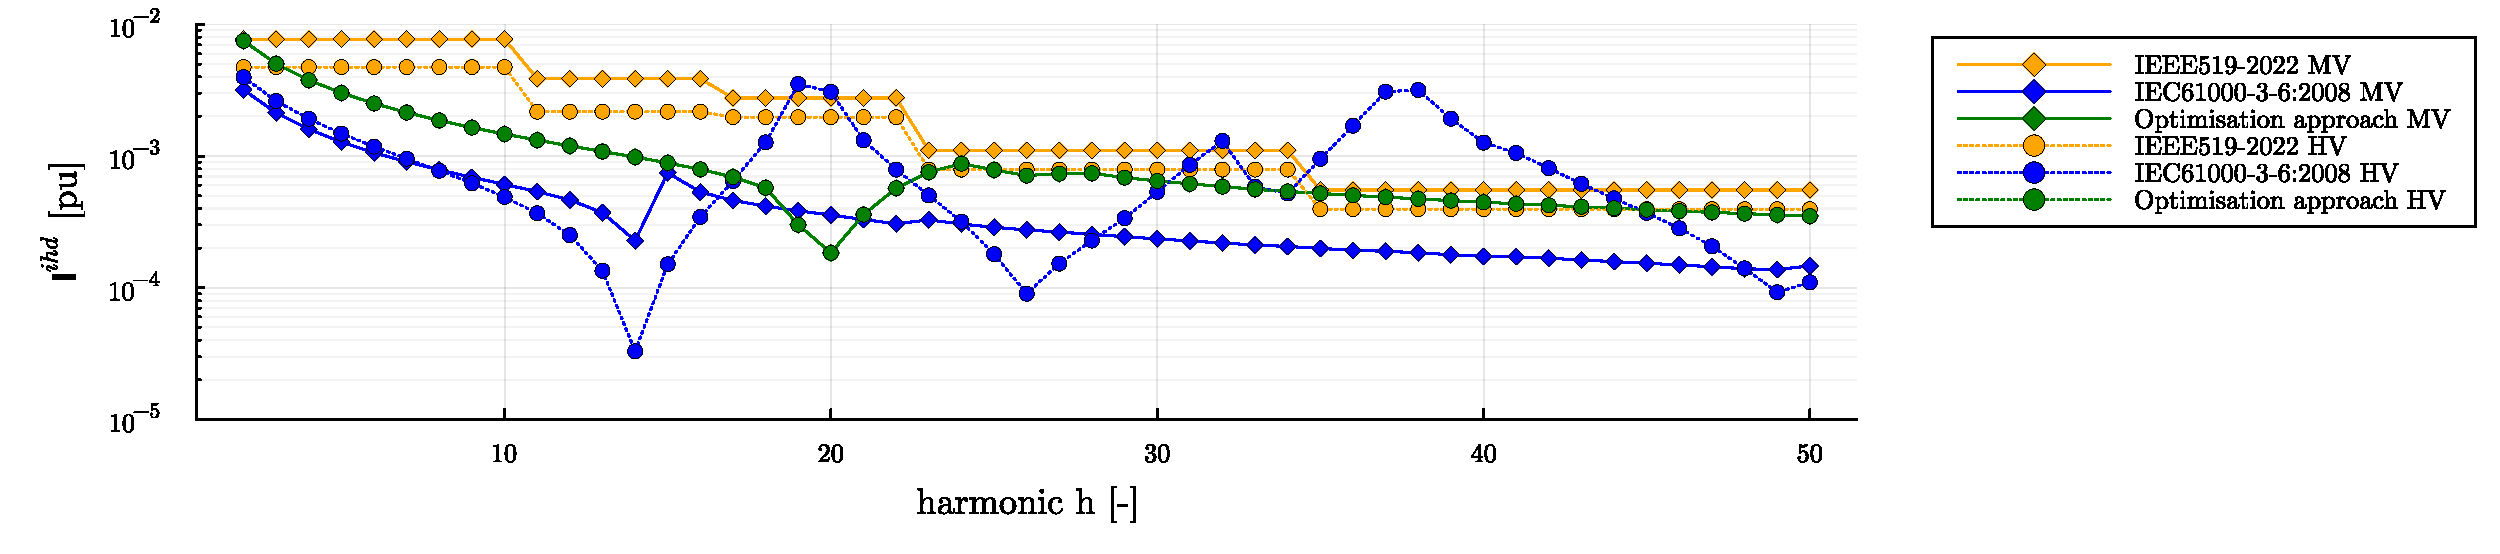
\includegraphics[height=3.5cm]{figures/ihd_cap.pdf}
\caption{Case B: underground cable network -- individual harmonic current~$\Current^{\text{ihd}}_{12,\Harmonic}$ of unit~12 at medium-voltage bus~17 (solid lines w. diamond marker) and~$\Current^{\text{ihd}}_{3,\Harmonic}$ unit~3 at high-voltage bus~4 (dotted lines w. circle marker), using one of three methods: a) IEEE519-2022 (orange), b) IEC61000-3-6:2008 (blue), and c) novel optimization method (green). Note that the curves for the optimization method (green) overlap due to the chosen absolute equality fairness principle.}
\label{fig:i_ihd_cap}
\end{figure*}

\begin{figure*}
\centering
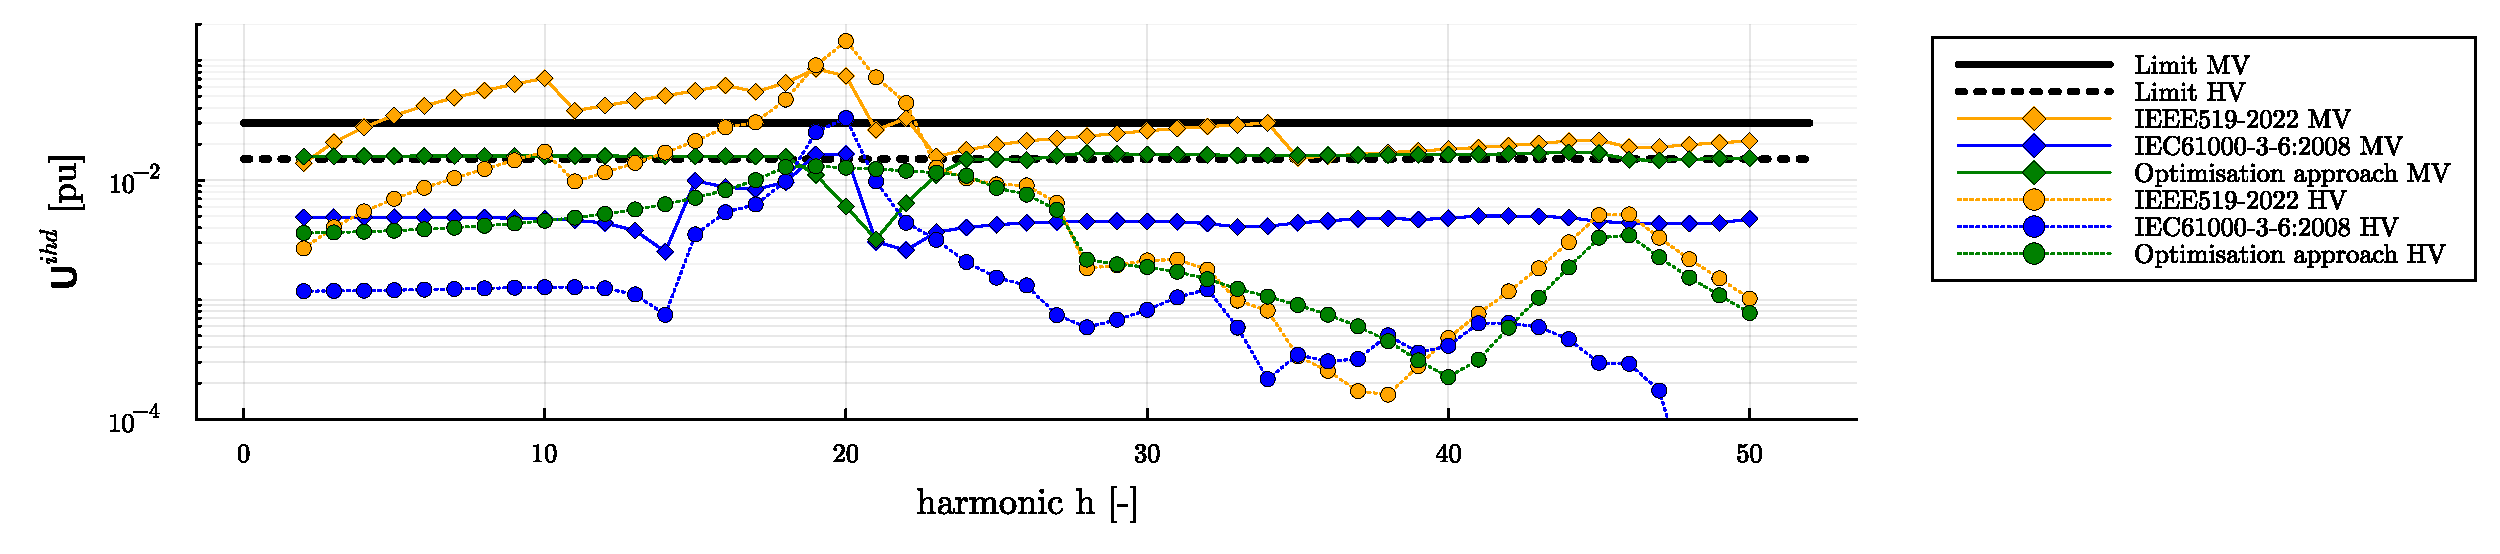
\includegraphics[height=3.5cm]{figures/uhd_cap.pdf}
\caption{Case B: underground cable network -- resulting individual harmonic voltage~$\Voltage^{\text{ihd}}_{17,\Harmonic}$ at medium-voltage bus~17 (solid lines w. diamond marker) and~$\Voltage^{\text{ihd}}_{4,\Harmonic}$ at high-voltage bus~4 (dashed lines w. circle marker), following a harmonic power flow based on the injected harmonic unit current determined using one of three methods: a) IEC61000-3-6:2008 (blue), b) IEEE519-2022 (orange), and c) novel optimization method (green).}
\label{fig:u_ihd_cap}
\end{figure*}

% This section presents the case study of the harmonic hosting capacity problem of a phase-balanced three-phase power system accounting for power system exploitation. As a test system we are using a modified version of the IEEE 30 bus test system, where we vary the impedance of the system to analyze the effect of the impedance on the permissible harmonic hosting capacity determined based both on the IEEE519-2022 and IEC61000-3-6:2008 standards as well as with the proposed hosting capacity optimization approach. The IEEE 30 bus test system consists of two distinct areas with voltage levels of 132~kV and 33~kV, respectively( as depicted in Figure~XXX (let's see if figure is necessary)). The IEEE 30 bus test system contains underground cables on the 132~kV level. We first convert these underground cables into overhead lines to start from a purely inductive system representation, and then successively convert the 132~kV connections back into underground cables shifting the the system impedance to capacitive values. Figure \ref{fig:impedance_scan} shows the resulting impedance scan of the network, seen from bus 8, which is located at the 132~kV level. As expected there are no parallel or series resonances in the range of the first 50 harmonics for the purely inductive system, and already after the addition of the first underground cable, resonances are observed in the frequency region of interest.

% \begin{figure}[ht]
% \centering
% 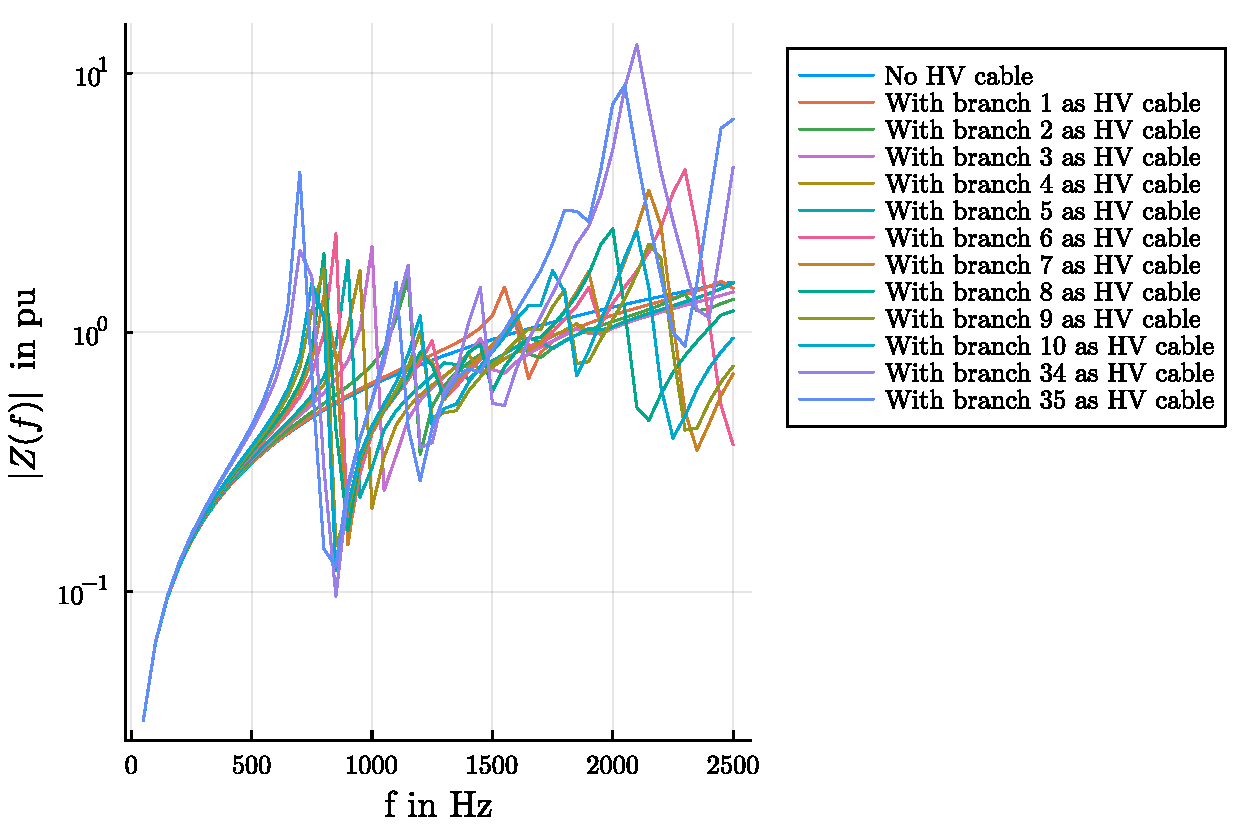
\includegraphics[width = \columnwidth]{figures/impedance_scan.pdf}
% \caption{Impedance scan of the modified IEEE 30 test system observed at bus 8 for different underground cables added to the system}
% \label{fig:impedance_scan}
% \end{figure}

% Next, we determine the harmonic hosting capacity based on the according to the standards, for which the results are depicted in Figure~XXXX (or table).  Note that for the determination of the hosting capacity based on IEC61000-3-6:2008 an equal amount of admissible harmonic current injections for each bus have been assumed, which means that admissible hosting capacity is determined by the most constrained bus, e.g. the bus with the highest harmonic impedance. The figure also shows that there are significant difference between the both standards with respect to the permissible harmonic hosting capacity. Figure~XX depicts the harmonic hosting capacity determined with the proposed optimization approach. We can observe that the available hosting capacity is significantly lower than (add exact value) the calculation based on the standards, i.e., the standards tend to over estimate the harmonic budget. To that end for the calculation based on IEC61000-3-6:2008, Figure~xxx also shows cases where a harmonic budget in percentage of the admissible individual injection is allocated for each bus, accounting for the effect simultaneous injections at other locations in the grid.  

% \begin{figure}[ht]
% \centering
% 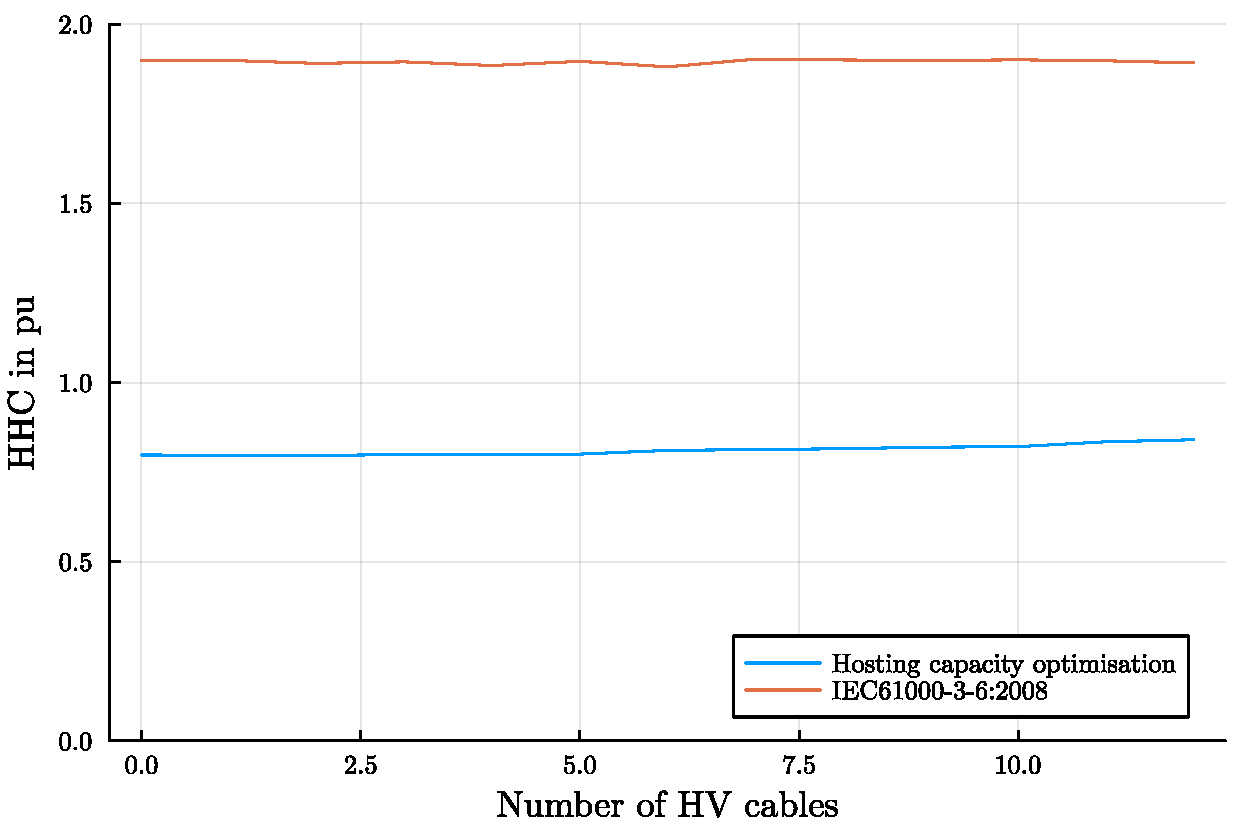
\includegraphics[width = \columnwidth]{figures/hosting_capacity.pdf}
% \caption{Harmonic hosting capacity calculated according to IEC61000-3-6:2008 and based on the optimization approach}
% \label{fig:hosting_capacity}
% \end{figure}







